\documentclass[12pt]{article}

\usepackage[french]{babel}
%\usepackage[latin1]{inputenc}
%\usepackage[english]{babel}

\usepackage{aeguill}
\usepackage{amsmath}
\usepackage{appendix}
\usepackage{color}
\usepackage{comment} % commenting out parts
\usepackage{epsfig}
\usepackage{euscript}
\usepackage{fancyhdr}
\usepackage[T1]{fontenc}
\usepackage{graphicx}
\usepackage[charter]{mathdesign}
\usepackage{amssymb}
\usepackage{latexsym}
\usepackage{listings}
\usepackage{multicol}
\usepackage{multirow}
\usepackage{pstricks}
\usepackage{subcaption}
\usepackage{theorem}
\usepackage{array}
\usepackage{url}
\setlength\extrarowheight{2pt}

\DeclareGraphicsExtensions{.pdf, .jpg, .png , .bmp}

{\theorembodyfont{\rmfamily}
\newtheorem{exo}{Exercice}
\newtheorem{exob}{Exercice}}

\newtheorem{Def}{D\'efinition}
\newtheorem{Defs}{\translation{D\'efinitions}}
\newtheorem{Rem}{Remarque}
\newtheorem{Prop}{Propri\'et\'e}
\newtheorem{exemple}{\sl Exemple }
%\pagestyle{empty}

\setlength{\voffset}{-2cm}\addtolength{\textheight}{4cm}
\setlength{\hoffset}{-1.7cm}\addtolength{\textwidth}{3.4cm}

\def\N{{\mathbb N}}
\def\R{{\mathbb R}}
\def\Z{{\mathbb Z}}
\def\p{{\hbox{P}}}
\def\e{{\hbox{E}}}
\def\un#1{{\hbox{\bf\large 1}}_{\scriptstyle #1}}

\setlength{\itemsep}{1mm} \setlength{\parsep}{0mm}
\newtheorem{theo}{Th\'eor\`eme}
\def\bt{\begin{theo}}
\def\ft{\end{theo}\par{} \vspace{3mm}}
\renewcommand{\theenumi}{\arabic{enumi})}
\renewcommand{\labelenumi}{\theenumi}
\renewcommand{\theenumii}{\alph{enumii}}
\renewcommand{\labelenumii}{\theenumii.}

\definecolor{commentcolor}{RGB}{145, 145, 145}
\definecolor{keywordcolor}{RGB}{139,0,0}
\definecolor{digitcolor}{RGB}{28, 28, 28}
\definecolor{numbercolor}{RGB}{28,28, 28}
\definecolor{stringcolor}{RGB}{60,179,113}
\definecolor{backcolour}{RGB}{247, 247, 247}
\definecolor{codecolor}{RGB}{28, 28, 28}
%\definecolor{functioncolor}{RGB}{186,85,211}


\begin{document}
	
	\thispagestyle{empty}
	\setcounter{page}{0}
		%\pagestyle{empty}
	\begin{center}
		%\begin{figure}[h!]
		\begin{tabular}{lcc}
			\centering
			%\hspace{-2cm}
			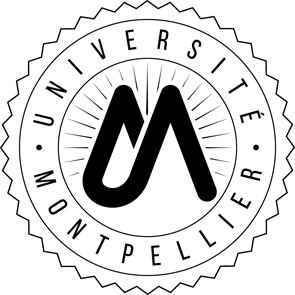
\includegraphics [height = 2cm]{logo-um}
			\hspace{1cm}
			%\end{figure}
			&
			\centering
			\begin{tabular}{c}
				{\huge Universit\'e de Montpellier}\\
				{\huge Facult\'e des Sciences}
			\end{tabular}
			&
			\hspace{1cm}
			\hfill \hfill
			\centering
			
\includegraphics [height = 2cm]{logo-fds}
		\end{tabular}
	\end{center}

\noindent\hrulefill\vspace{3mm}\par
\vspace{5cm}

\begin{center}
	{\Large{	{ Projet Mod\`eles Linéaires Avancées} }} \\
	
	\vspace{1cm}
	
	{\Large{ {\bf  Ryma Lakehal }}} \\
\end{center}

\vspace{10cm}
\noindent\hrulefill\vspace{3mm}\par

{\sc{M2 MIND}} 	\hfill \hfill     2020-2021 \\

%%%%%%%%%%%%%%%%%%%%%%%%%%%%%%%%%%%%%%%%%%
 \newpage
 \tableofcontents
 
\newpage
%\thispagestyle{fancy}
%%%%%%%%%%%%%%%%%%%%%%%%%%%%%%%%%%%%%%%%%%

\section{Introduction}

    Les GLM (modèles linéaires généralisés) sur données de comptage, régression de Poisson ou regression binomiale négative, sont des approches statistiques qui doivent être employées lorsque la variable à analyser résulte d’un processus de comptage. Ces approches sont indispensables, car dans cette situation les hypothèses des modèles linéaires classiques ne sont plus satisfaites (Les données de comptage diffèrent des données avec une erreur normale de plusieurs façons, y compris 1) les comptages sont discrets et peuvent être des nombres entiers nuls ou positifs seulement, 2) les comptages ont tendance à se regrouper sur le petit côté de la plage, créant une distribution avec un biais positif , 3) un échantillon de dénombrements peut avoir une abondance de zéros, et 4) la variance des dénombrements augmente avec la moyenne).
    
    De manière plus précise, les modèles de régression de Poisson (resp.binomiale négative), sont des GLM, comportant une fonction de lien log et une structure d’erreur de type Poisson (resp.binomiale négative).
    
    Dans cet article, Nous allons mettre en oeuvre ces approches, avec Python sur les données "L'approvisionnement en sucre maximise le service de biocontrôle des parasitoïdes"
    
    
    \subsection{Présentation des données \texttt{Parastism}}
    Pour déterminer si les provisions de sources de sucre augmente le parasitisme de l'Aphytis,  le parasite actif a été calculé pour trois traitements, ainsi que le nombre de parasitées éliminés pendant le test.
    Parmi 288 fruit collectés, 196 fruits contient au moins un parasitoïde vivant ou éradiqué (63 fruits non infectés "contrôlés", 67 fruits avec le parasite \textit{A. melinus} sans sucre et 66 fruits infectés du même parasite plus le sucre). Au total, il a été enregistré 949 parasitoïdes vivants et 365 parasites éliminés contenant un œuf ou larves d'Aphytis. 
    

    
\begin{figure}[h]
\centering
 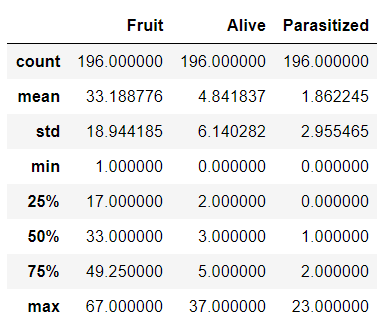
\includegraphics[width=.45\textwidth]{datadescribe.png}
 \caption{Le jeu de données \texttt{Parastism }} 
 \end{figure}
 
 \begin{figure}[h]
\centering
 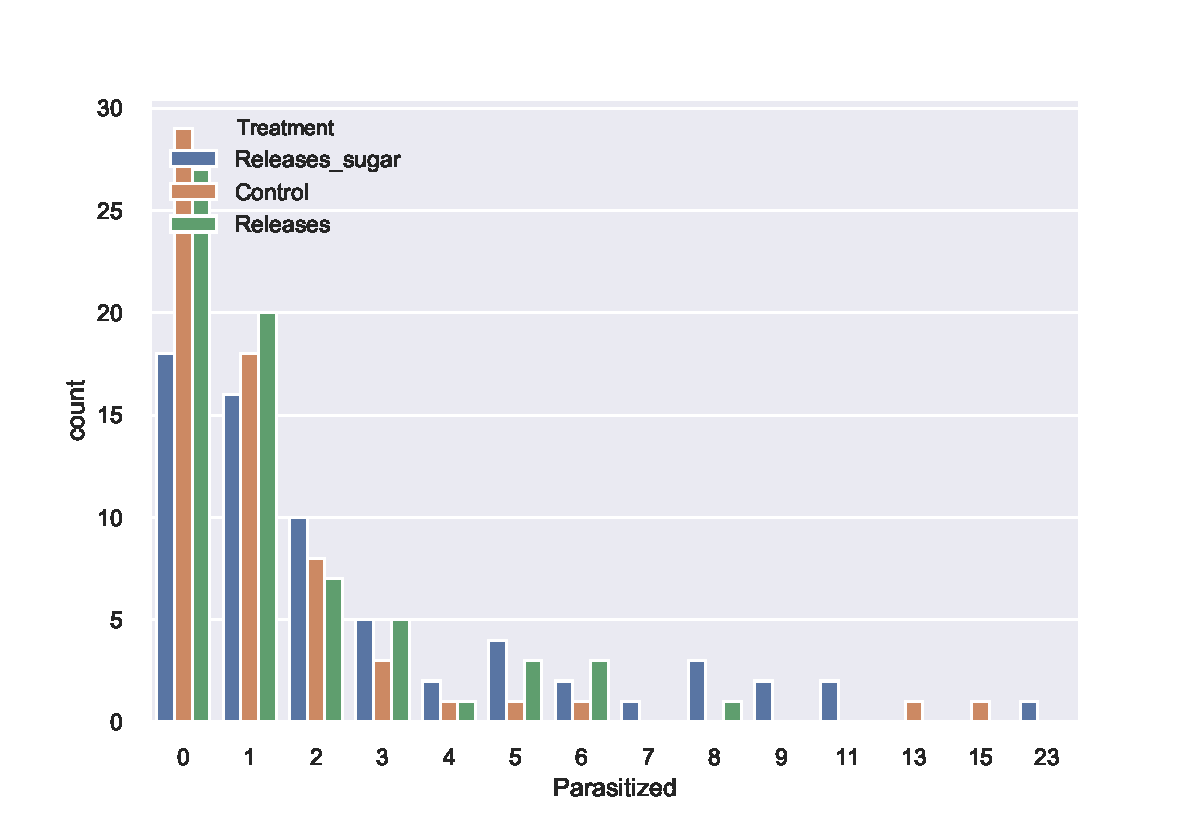
\includegraphics[width=1\textwidth]{Histogram of the count.pdf}
 \caption{Histogramme des traitements en fonction de la variable \texttt{Parasitized} } 
 \label{hist_para}
 \end{figure}
 
 La figure \ref{hist_para} montre que les données de comptages sont entassées pour la majorité d'un seul côté de l'histogramme et qu'au moins un tiers de chaque traitement est égale à zero.


\newpage
~
\newpage
\section{Le modèle linéaire généralisé}
une façon courante dont les chercheurs en biologie pensent pour modéliser la variable à expliquer est

\begin{align*}
y_i &= \beta_0 + \beta_1 x_i + \varepsilon_i \\
\varepsilon &\sim N(0, \sigma)
\tag{1}
\end{align*}

mais ces modèles classiques ne sont pas adaptés pour analyser des variables à expliquer (ou réponses) de type “comptage”, notamment parce qu’ils supposent que celles-ci sont distribuées selon une loi Normale. Cette hypothèse conduit alors à considérer que la variance des résidus est homogène, autrement dit constante, quelle que soit la valeur des comptages moyens prédits par le modèle. Or, les données de type comptage ne sont pas distribuées selon une loi Normale, mais selon une loi de Poisson. Et compte tenu de cette loi de distribution ,la variance des résidus n’est pas constante mais proportionnelle aux comptages moyens prédits par le modèle.
Par exemple, si on veut modéliser le nombre de parasites qui ont infectés les fruits ce serait plus adapté d'utiliser la distribution de Poisson.

\begin{align*}
y_i &\sim N(\mu_i, \sigma)\\
\mathrm{E}(Y|X) &= \mu\\
\mu_i &= \beta_0 + \beta_1 x_i
\tag{2}
\end{align*}
La spécification d'un modèle linéaire généralisé comporte à la fois des parties stochastiques et systématiques, mais en ajoute une troisième, qui est une fonction de lien reliant les parties stochastique et systématique.
\begin{itemize}
    \item La partie stochastique, qui est une distribution de probabilité de la famille exponentielle
    \begin{equation*}
    y_i \sim \mathrm{Prob}(\mu_i)
    \end{equation*}
    \item la partie systématique, qui est un prédicteur linéaire
    \begin{equation*}
    \eta=\mathbf{X}\boldsymbol{\beta}
    \end{equation*}
    \item une fonction de liaison reliant les deux parties
    \begin{equation*}
    \eta_i = g(\mu_i)
    \end{equation*}
\end{itemize}

Cependant, contrairement aux modèles linéaires classiques, les valeurs prédites par le prédicteur linéaire du GLM ne correspondent pas à la prédiction moyenne d’une observation, mais à la transformation (par une fonction mathématique) de celle-ci. Dans le cas de la régression de Poisson il s’agit de la transformation log.

Pour obtenir la prédiction moyenne, il est alors nécessaire d’appliquer la fonction inverse du Log, c’est à dire la fonction exponentielle

\section{Exemple de données de comptage}
Sur les données \texttt{Parastism} mesurant l'effet des traitements (\texttt{Control} , \texttt{Realises\_sugar} et \texttt{Realises}) sur les arbres/fruits.

\subsection{Stratégie de modélisation}
Nous allons d'abord ajusté le modèle et ensuite nous allons vérifier ses hypothèses à l'aide des graphique de diagnostic.\\
Commençons par le modèle linéaire classique pour illustrer et interpréter les graphiques dans le cas des données non gaussiennes.\\
Le modèle :
\begin{align*}
Parasitized_i &= \beta_0 + \beta_1 Control_i + \beta_2 Realises_i + \beta_3 Realises\_sugar_i + \varepsilon_i \\
\varepsilon &\sim N(0, \sigma)
\tag{3}
\end{align*}

\subsection{Normlité - Q-Q plot normal}

L'histogramme montre que les résidus sont négatives, ce qui suggère que le modèle avec un bruit gaussien n'est pas bien ajusté.

\begin{figure}[h]
\centering
 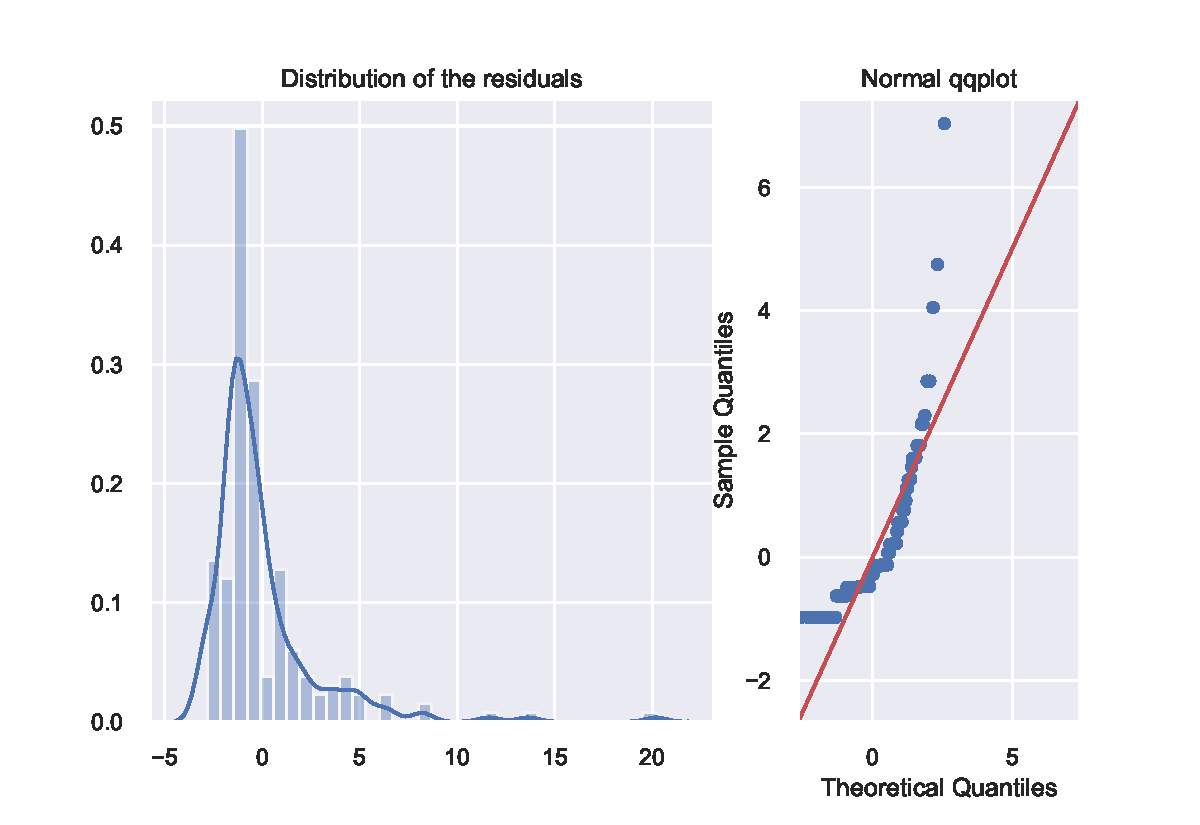
\includegraphics[width=1\textwidth]{Distribution and normal QQ plot residuals .pdf}
 \caption{Distribution et normal Q-Q plot des résidus du modèle linéaire ajusté} 
 \label{norm_qq}
 \end{figure}

Ainsi que le Q-Q plot normal, qui trace les quantiles observés contre les quantiles théoriques, nous pouvons que les données \texttt{Parastism} ne sont pas normales car les points ne suivent pas la ligne rouge. 

\subsection{Homoscédasticité - scale-location plot}
\begin{figure}[h]
\centering
 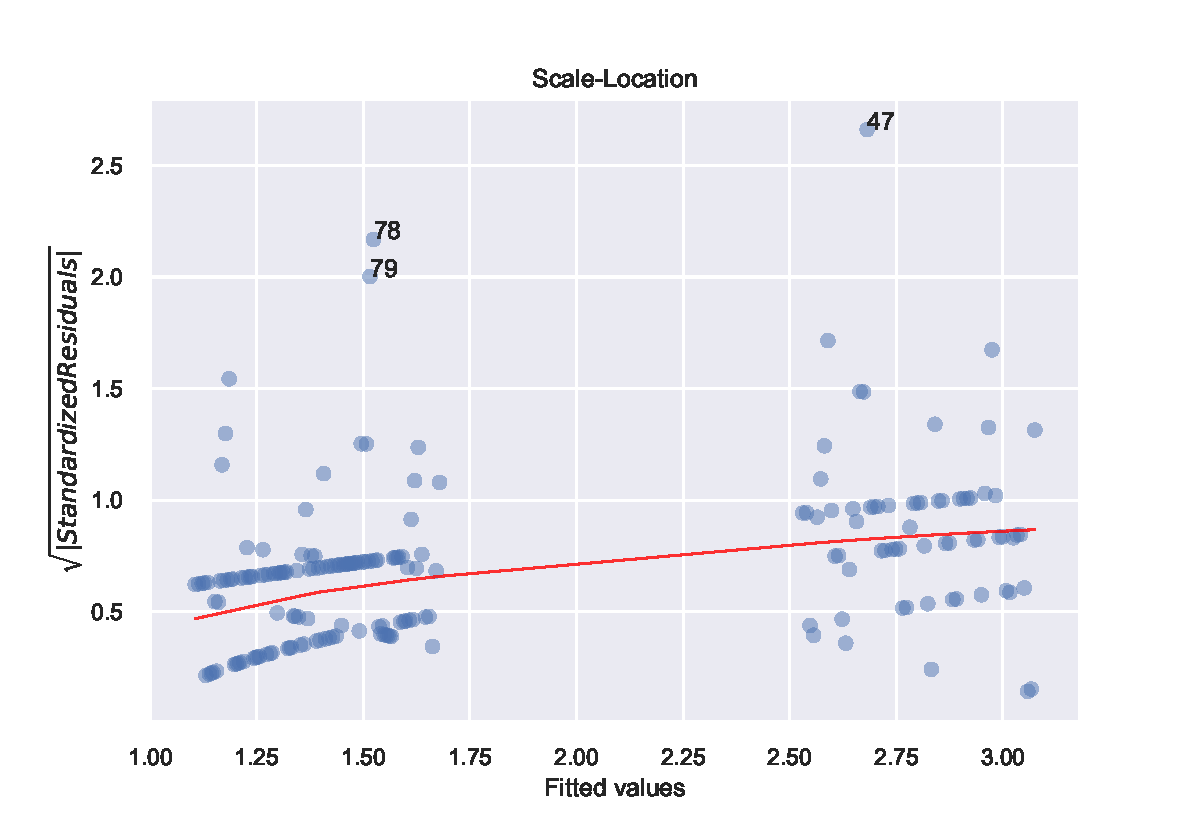
\includegraphics[width=1\textwidth]{scale-location plot.pdf}
 \caption{scale-location plot pour vérifier l'homoscédasticité} 
 \label{homosc}
 \end{figure}
 
 Un modèle linéaire a aussi pour hypothèse l'homoscédasticité des résidus. Sur la figure \ref{homosc}, nous pouvons voir que le bruit n'est pas homoscédastique. En effet,la droite de régression n'est pas horizontale (ou proche de l'horizontale), elle est plutôt croissante, ce qui est attendu que les données soient de distribution de Poisson, Binomiale  négative ou logNormales.
 
 \section{Régression de Poisson}
 On dit qu’une variable aléatoire Y suit une distribution de Poisson de paramètre Lambda, si elle prend pour valeur y = 0 ,1,2,3,… avec une probabilité P définie par :
 
 $$
 P({Y=y}) = \frac{e^{-\lambda}\; \lambda^y}{y\;!}
 $$
 La distribution de Poisson est ainsi définie par un seul paramètre : Lambda. Pour fixer les idées, voici quelques exemples de distribution, pour des valeurs de Lambda variant entre 1 et 30.
 
 \begin{figure}[h]
\centering
 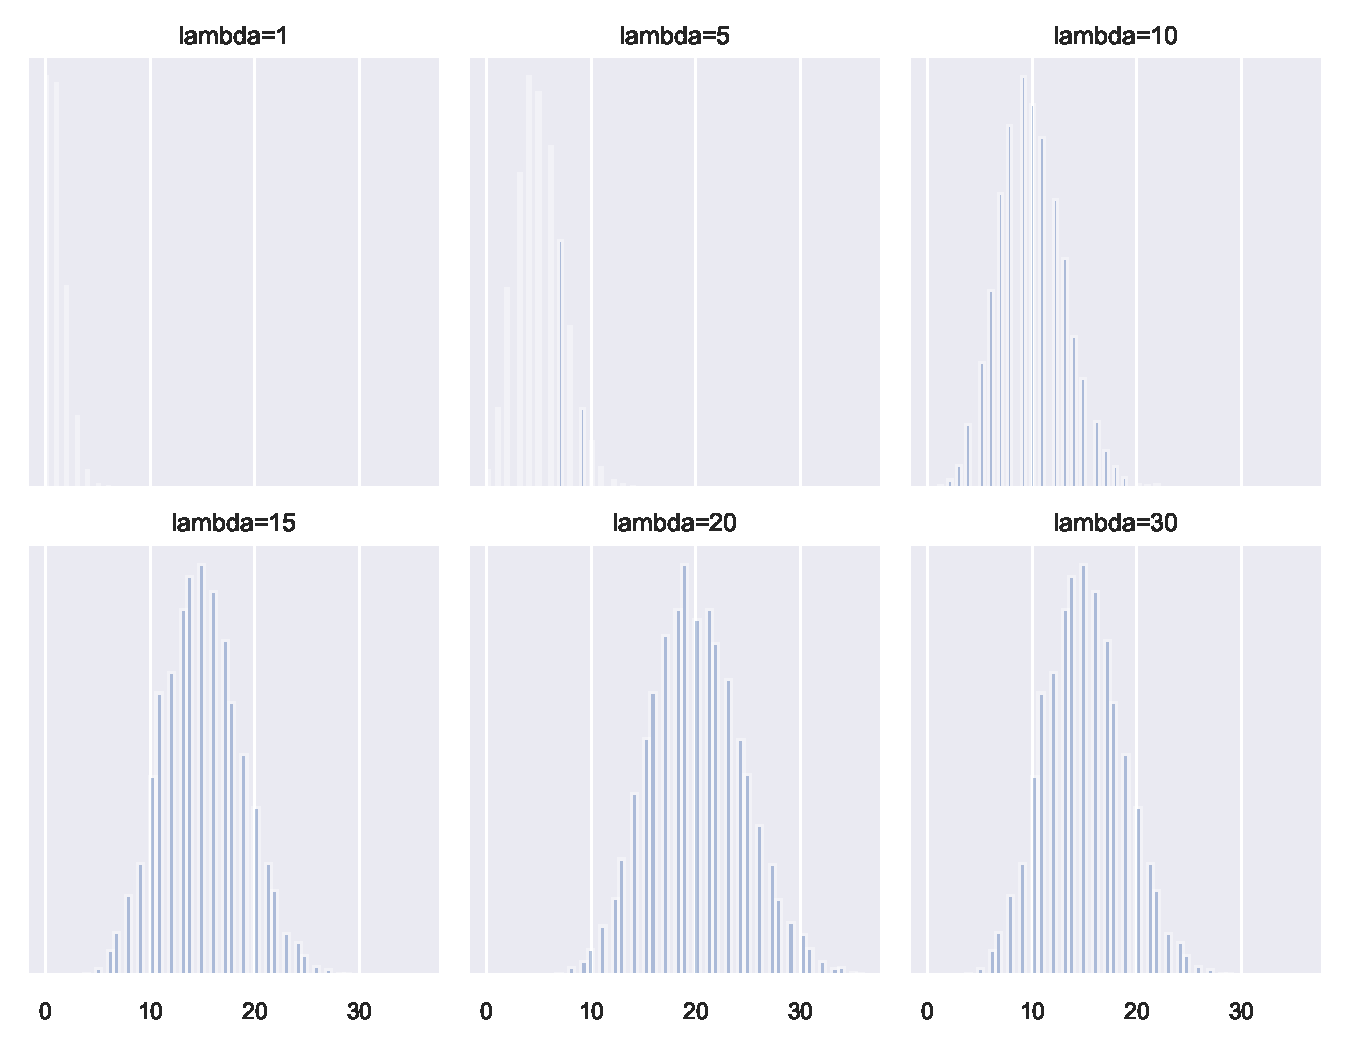
\includegraphics[width=.8\textwidth]{histogram poisson dist.pdf}
 \caption{La distribution de Poisson} 
 \label{poiss_dist}
 \end{figure}

Plus $\lambda$ augmente, plus la distribution de Poisson se rapproche d’une loi Normale (cf. \ref{poiss_dist}) 

\subsection{Ajustement du modèle de régression linéaire de Poisson aux données \texttt{Parastism}}

Le modèle est : 

\begin{align*}
Parasitized_i &\sim Poisson(\mu_i)\\
\mathrm{E}({Parasitized|Treatment}) &= \mu\\
\mu_i &= \mathrm{exp}(\eta_i)\\
\eta_i &= \beta_0 + \beta_1 Control_i + \beta_2 Realises_i + \beta_3 Realises\_sugar_i
\end{align*}



L’ajustement est réalisé à l’aide de la fonction \textbf{Poisson.fit} du module \textbf{statsmodels}


\lstset{
basicstyle=\fontsize{8}{11}\selectfont\ttfamily,
backgroundcolor=\color{backcolour}
}
\begin{lstlisting}[caption=Python-output from fitting a GLM to count data]
                 Generalized Linear Model Regression Results                  
==============================================================================
Dep. Variable:            Parasitized   No. Observations:                  196
Model:                            GLM   Df Residuals:                      193
Model Family:                   Gamma   Df Model:                            2
Link Function:          inverse_power   Scale:                          2.4206
Method:                          IRLS   Log-Likelihood:                    inf
Date:                Fri, 30 Oct 2020   Deviance:                       5304.4
Time:                        03:51:41   Pearson chi2:                     467.
No. Iterations:                     8                                         
Covariance Type:            nonrobust                                         
==================================================================================================
                                     coef    std err          z      P>|z|      [0.025      0.975]
--------------------------------------------------------------------------------------------------
Intercept                          0.7326      0.144      5.102      0.000       0.451       1.014
C(Treatment)[T.Releases]          -0.0198      0.197     -0.100      0.920      -0.407       0.367
C(Treatment)[T.Releases_sugar]    -0.3758      0.159     -2.363      0.018      -0.687      -0.064
==================================================================================================
 
 \end{lstlisting}

Les valeurs \texttt{coef} sont les estimations des paramètres $\beta$. La modalité \texttt{Control} est choisi comme modalité de référence (Intercept).
Les modalités \textbf{Intercept} et \textbf{Realises\_sugar} ont un effet significative au developpement des parasoïdes au risque d'erreur 5\%
 
 
 Le ratio residual deviance / ddl est égal à 5304.4 /193, soit 27,48. Ce ratio est très largement supérieur à 1 et permet de mettre en évidence la présence d’une surdispersion. Il est donc nécessaire d’utiliser une autre structure d’erreur dans le modèle de régression. ce qui est souvent le cas dans pour les données de comptage biologique. Une distribution utile pour les données de comptage avec surdispersion est la binômiale négative.
 
 \section{Régression binomiale négative}
On fait pareillement pour la régression binomiale négative :

\subsection{Ajustement du modèle de régression binomiale négative aux données \texttt{Parastism}}

\begin{align*}
Parasitized_i &\sim NB(\mu, k)\\
\mathrm{E}({Parasitized|Treatment}) &= \mu\\
\mu_i &= \mathrm{exp}(\eta_i)\\
\eta_i &= \beta_0 + \beta_1 Control_i + \beta_2 Realises_i + \beta_3 Realises\_sugar_i
\end{align*}

\begin{lstlisting}[caption=Python-output from fitting a GLM to count data]
                 Generalized Linear Model Regression Results                  
==============================================================================
Dep. Variable:            Parasitized   No. Observations:                  196
Model:                            GLM   Df Residuals:                      193
Model Family:        NegativeBinomial   Df Model:                            2
Link Function:                    log   Scale:                          1.0000
Method:                          IRLS   Log-Likelihood:                -355.42
Date:                Sat, 07 Nov 2020   Deviance:                       228.53
Time:                        22:45:25   Pearson chi2:                     290.
No. Iterations:                     5                                         
Covariance Type:            nonrobust                                         
==================================================================================================
                                     coef    std err          z      P>|z|      [0.025      0.975]
--------------------------------------------------------------------------------------------------
Intercept                          0.3112      0.166      1.877      0.061      -0.014       0.636
C(Treatment)[T.Releases]           0.0274      0.230      0.119      0.905      -0.424       0.479
C(Treatment)[T.Releases_sugar]     0.7195      0.219      3.282      0.001       0.290       1.149
==================================================================================================

\end{lstlisting}
 
Ici, les modalités \textbf{Intercept} et \textbf{Realises} ont un effet significative au developpement des parasoïdes au risque d'erreur 5\%, et le ratio residual deviance / ddl est égal à 1.18, proche de 1.

\subsection{Calculs des effets marginaux}
Les effets marginaux sont une métrique alternative qui peut être utilisée pour décrire l'impact d'un prédicteur sur la variable à expliquer. Les effets marginaux peuvent être décrits comme le changement du résultat en fonction du changement du traitement maintenant toutes les autres variables du modèle comme des constantes.\\
On s'intéresse aux effects marginaux à la moyenne, pour ce faire, on a la fonction \textbf{.get\_margeff()} de la bibliothèque \textbf{Statsmodels}.


\begin{lstlisting}[caption=Python-output Marginal effects]
  NegativeBinomial Marginal Effects  
=====================================
Dep. Variable:            Parasitized
Method:                          dydx
At:                              mean
==================================================================================================
                                    dy/dx    std err          z      P>|z|      [0.025      0.975]
--------------------------------------------------------------------------------------------------
C(Treatment)[T.Releases]           0.0481      0.438      0.110      0.913      -0.811       0.907
C(Treatment)[T.Releases_sugar]     1.2632      0.429      2.948      0.003       0.423       2.103
==================================================================================================
\end{lstlisting}

La valeur de \textbf{Releases\_sugar} est 1.26 ce qui peut être interprété que quand la valeur de \textbf{Releases\_sugar} augmente d'une unité, la probabilité des parasitoïdes éliminé ou le taux de parasitism augmente de 126\%. 

\section{Conclusion}
En effect, ça a été démontré que les provisions de sucre peut aider les parasitoïdes à maintenir leurs réserves de sucre, à augmenter la fécondité et ainsi augmente les taux de parasitisme, ce qui est concordant avec les résultats que nous avons obtenus.


\end{document}